
\documentclass[12pt,a4paper]{article}

% Pacotes
\usepackage[utf8]{inputenc}
\usepackage[T1]{fontenc}
\usepackage[brazil]{babel}
\usepackage{amsmath}
\usepackage{amssymb}
\usepackage{geometry}
\usepackage{booktabs}
\usepackage{array}
\usepackage{graphicx}
\usepackage{microtype}
\usepackage{enumitem}

% Configurações
\geometry{a4paper, margin=2.5cm}
\setlength{\parindent}{1.25cm}
\setlength{\parskip}{0.4em}
\setlist[itemize]{nosep, topsep=0.4em}
\renewcommand{\arraystretch}{1.2}
\widowpenalty=10000
\clubpenalty=10000
\setlength{\emergencystretch}{1em}

\usepackage{float}
\begin{document}

\begin{center}
    {\Large \textbf{Otimização Combinatória}}\\[0.3cm]
    {\large Trabalho -- Tema 4: Radioterapia}\\[0.2cm]
    \textbf{Modelagem, solução e análise de sensibilidade}
\end{center}

\vspace{0.5cm}

\section*{Tarefa 1 -- O Modelo}

\subsection*{Item (a)}

\textbf{Por que a dose numa região é uma soma de termos
do tipo coeficiente $\times$ intensidade?
Que hipótese física está por trás?}

\subsubsection*{Resposta}

A dose total de radiação recebida por uma região é
calculada pela soma das contribuições de cada feixe.

Cada contribuição é obtida multiplicando a intensidade
do feixe pelo coeficiente que representa a dose
depositada naquela região por unidade de intensidade.

A hipótese física utilizada é a
\textbf{linearidade e a superposição das doses},
ou seja, considera-se que a dose depositada por cada
feixe é proporcional à sua intensidade e que as
contribuições dos diferentes feixes podem ser somadas.

\subsubsection*{Explicação}

O tratamento utiliza quatro feixes de radiação:

\begin{itemize}
    \item \textbf{A:} Feixe anterior;
    \item \textbf{B:} Feixe posterior;
    \item \textbf{C:} Feixe lateral esquerdo;
    \item \textbf{D:} Feixe lateral direito.
\end{itemize}

Cada feixe deposita uma quantidade diferente de
radiação em cada região do corpo.

Na borda do tumor, os coeficientes são:

\begin{center}
\begin{tabular}{cc}
\toprule
\textbf{Feixe} & \textbf{Dose por unidade de intensidade} \\
\midrule
A & 0,6 Gy \\
B & 0,5 Gy \\
C & 0,9 Gy \\
D & 0,4 Gy \\
\bottomrule
\end{tabular}
\end{center}

Assim, a dose na borda do tumor é representada por:

\[
D_{\text{borda}} =
0{,}6x_A + 0{,}5x_B + 0{,}9x_C + 0{,}4x_D
\]

Por exemplo, considerando que todos os feixes
possuam intensidade igual a 10:

\[
D_{\text{borda}} =
0{,}6(10) + 0{,}5(10) + 0{,}9(10) + 0{,}4(10)
\]

\[
D_{\text{borda}} = 6 + 5 + 9 + 4
\]

\[
\boxed{D_{\text{borda}} = 24\text{ Gy}}
\]

Portanto, os quatro feixes juntos depositariam
24 Gy na borda do tumor.

O modelo é linear porque, ao dobrar a intensidade
de um feixe, sua contribuição para a dose também
dobra. Além disso, a contribuição de cada feixe
é considerada independente das demais.

\newpage

\subsection*{Item (b)}

\textbf{Escreva o Problema de Programação Linear
(PPL) com as intensidades
$x_A$, $x_B$, $x_C$ e $x_D$,
minimizando a dose média no tecido sadio,
respeitando as exigências da tabela.}

\subsubsection*{Passo 1 -- Variáveis de decisão}

As variáveis de decisão representam as intensidades
dos quatro feixes de radiação:

\begin{align*}
x_A &= \text{Intensidade do feixe anterior} \\
x_B &= \text{Intensidade do feixe posterior} \\
x_C &= \text{Intensidade do feixe lateral esquerdo} \\
x_D &= \text{Intensidade do feixe lateral direito}
\end{align*}

Todas as variáveis devem ser não negativas,
pois não existem intensidades negativas de radiação.

\subsubsection*{Passo 2 -- Função objetivo}

O objetivo do problema é minimizar a dose média
de radiação depositada no tecido sadio.

Os coeficientes fornecidos são:

\begin{center}
\begin{tabular}{cc}
\toprule
\textbf{Feixe} & \textbf{Dose média por unidade} \\
\midrule
A & 0,04 Gy \\
B & 0,05 Gy \\
C & 0,08 Gy \\
D & 0,06 Gy \\
\bottomrule
\end{tabular}
\end{center}

A função objetivo é:

\[
\boxed{
\min Z =
0{,}04x_A + 0{,}05x_B +
0{,}08x_C + 0{,}06x_D
}
\]

Em que $Z$ representa a dose média
no tecido sadio, medida em Gy.

Busca-se encontrar as intensidades que produzam
a menor dose possível no tecido sadio,
sem comprometer o tratamento do tumor.

\subsubsection*{Passo 3 -- Restrições}

\paragraph{Restrição 1 -- Borda do tumor}

A borda do tumor deve receber pelo menos
60 Gy e no máximo 66 Gy.

\[
0{,}6x_A + 0{,}5x_B +
0{,}9x_C + 0{,}4x_D \geq 60
\]

\[
0{,}6x_A + 0{,}5x_B +
0{,}9x_C + 0{,}4x_D \leq 66
\]

\paragraph{Restrição 2 -- Centro do tumor}

O centro do tumor também deve receber uma dose
entre 60 Gy e 66 Gy.

\[
0{,}6x_A + 0{,}6x_B +
0{,}5x_C + 0{,}4x_D \geq 60
\]

\[
0{,}6x_A + 0{,}6x_B +
0{,}5x_C + 0{,}4x_D \leq 66
\]

\paragraph{Restrição 3 -- Medula espinhal}

A medula espinhal pode receber no máximo 45 Gy.

\[
0{,}2x_A + 0{,}6x_B +
0{,}2x_C + 0{,}2x_D \leq 45
\]

\paragraph{Restrição 4 -- Pulmão}

A dose média no pulmão não pode ultrapassar 20 Gy.

\[
0{,}3x_A + 0{,}1x_B +
0{,}8x_C + 0{,}1x_D \leq 20
\]

\paragraph{Restrição 5 -- Não negatividade}

As intensidades dos feixes não podem ser negativas.

\[
x_A, x_B, x_C, x_D \geq 0
\]

\newpage

\subsection*{Modelo matemático completo}

O Problema de Programação Linear é definido por:

\begin{equation*}
\boxed{
\begin{aligned}
\min \quad Z ={}&
0{,}04x_A + 0{,}05x_B +
0{,}08x_C + 0{,}06x_D
\end{aligned}
}
\end{equation*}

Sujeito a:

\begin{align*}
0{,}6x_A + 0{,}5x_B + 0{,}9x_C + 0{,}4x_D
&\geq 60
\\
0{,}6x_A + 0{,}5x_B + 0{,}9x_C + 0{,}4x_D
&\leq 66
\\
0{,}6x_A + 0{,}6x_B + 0{,}5x_C + 0{,}4x_D
&\geq 60
\\
0{,}6x_A + 0{,}6x_B + 0{,}5x_C + 0{,}4x_D
&\leq 66
\\
0{,}2x_A + 0{,}6x_B + 0{,}2x_C + 0{,}2x_D
&\leq 45
\\
0{,}3x_A + 0{,}1x_B + 0{,}8x_C + 0{,}1x_D
&\leq 20
\end{align*}

\[
\boxed{x_A,x_B,x_C,x_D \geq 0}
\]

\begin{figure}[H]
    \centering
    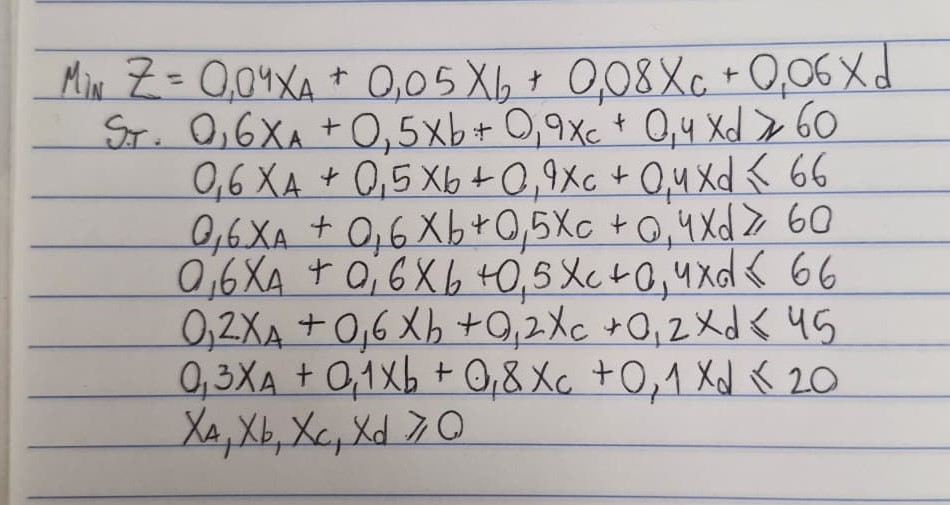
\includegraphics[width=0.8\linewidth]{Tarefa 1. ex A.jpeg}
    \caption{Modelo PPL feito à mão}
    \label{fig:modelo-manuscrito}
\end{figure}

\clearpage
\section*{Tarefa 2 -- O plano}

\begin{figure}[H]
    \centering
    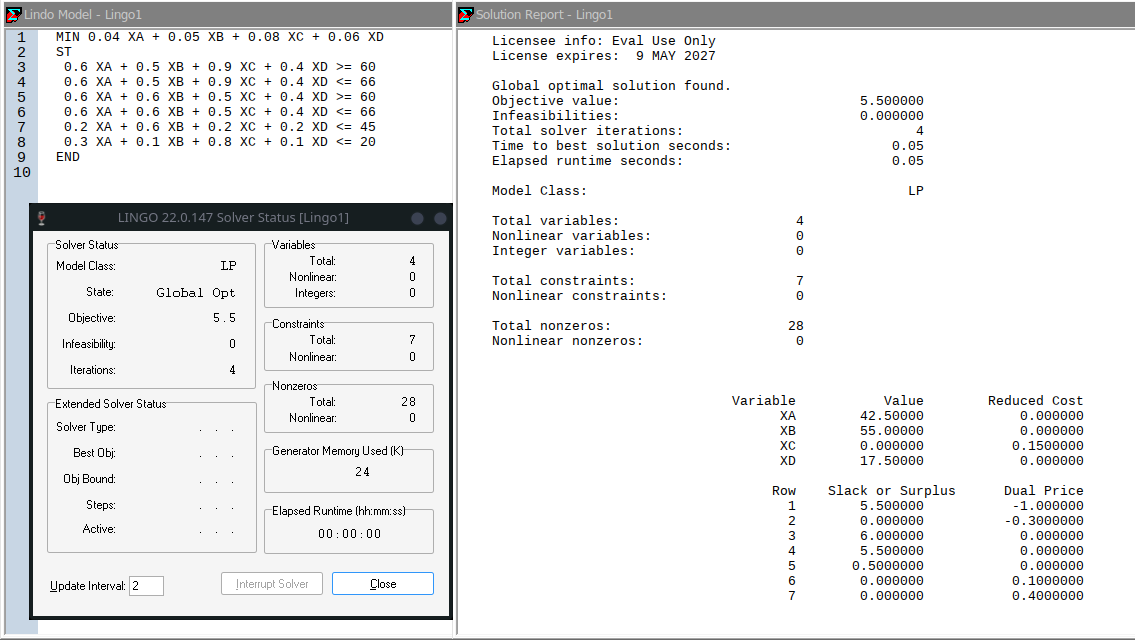
\includegraphics[width=0.8\linewidth]{Lindo tarefa 2.png}
    \caption{Execução do modelo PPL no LINDO}
    \label{fig:solucao-tarefa2}
\end{figure}

\subsection*{Item (a)}

\textbf{Qual a intensidade de cada feixe? Que feixe não é usado?}

As intensidades ótimas, apresentadas na coluna \texttt{Value} do
relatório, são $x_A=42{,}5$, $x_B=55$, $x_C=0$ e $x_D=17{,}5$
unidades de intensidade. Assim, o feixe anterior (A) tem intensidade
$42{,}5$, o posterior (B) tem intensidade $55$ e o lateral direito (D)
tem intensidade $17{,}5$.

\textbf{O feixe lateral esquerdo (C) não é usado}, pois sua intensidade
ótima é zero.

\subsection*{Item (b)}

\textbf{Calcule a dose em cada região. Quais exigências estão no limite?
Confira com a coluna \texttt{SLACK OR SURPLUS}.}

Substituindo as intensidades do item (a) nas expressões de dose, obtêm-se
\begin{align*}
D_{\text{borda}}
&=0{,}6(42{,}5)+0{,}5(55)+0{,}9(0)+0{,}4(17{,}5)
=60\text{ Gy},\\
D_{\text{centro}}
&=0{,}6(42{,}5)+0{,}6(55)+0{,}5(0)+0{,}4(17{,}5)
=65{,}5\text{ Gy},\\
D_{\text{medula}}
&=0{,}2(42{,}5)+0{,}6(55)+0{,}2(0)+0{,}2(17{,}5)
=45\text{ Gy},\\
D_{\text{pulmão}}
&=0{,}3(42{,}5)+0{,}1(55)+0{,}8(0)+0{,}1(17{,}5)
=20\text{ Gy},\\
D_{\text{sadio}}
&=0{,}04(42{,}5)+0{,}05(55)+0{,}08(0)+0{,}06(17{,}5)
=5{,}5\text{ Gy}.
\end{align*}

Conforme a tabela da seção ``O problema'' do enunciado
do trabalho, as doses no pulmão e no tecido sadio
representam doses médias. O valor de $5{,}5$ Gy corresponde ao mínimo da função objetivo.

\begin{center}
\begin{tabular}{clrr}
\toprule
\textbf{Linha} & \textbf{Exigência} & \textbf{Dose (Gy)} & \textbf{Folga (Gy)} \\
\midrule
2 & Borda $\geq 60$ Gy & $60$ & $0$ \\
3 & Borda $\leq 66$ Gy & $60$ & $6$ \\
4 & Centro $\geq 60$ Gy & $65{,}5$ & $5{,}5$ \\
5 & Centro $\leq 66$ Gy & $65{,}5$ & $0{,}5$ \\
6 & Medula $\leq 45$ Gy & $45$ & $0$ \\
7 & Pulmão $\leq 20$ Gy & $20$ & $0$ \\
\bottomrule
\end{tabular}
\end{center}

Os valores da última coluna conferem com \texttt{SLACK OR SURPLUS}
do relatório. Nas restrições de dose mínima, o excedente é a dose
recebida menos o mínimo exigido. Nas restrições de dose máxima,
a folga é o máximo permitido menos a dose recebida.

\textbf{Estão no limite a dose mínima na borda do tumor e as doses
máximas na medula espinhal e no pulmão}, pois as linhas 2, 6 e 7
apresentam folga zero. O centro recebe $65{,}5$ Gy, ficando
$5{,}5$ Gy acima do mínimo e $0{,}5$ Gy abaixo do máximo.

\clearpage
\section*{Tarefa 3 -- O preço de cada limite}

Como o problema é de minimização, melhorar o resultado significa diminuir
a dose média no tecido sadio. No plano original, essa dose é de $5{,}50$ Gy.
A coluna \textit{dual price} do relatório indica quanto o resultado melhora
quando aumentamos em uma unidade o limite de uma restrição, mantendo os
demais limites fixos. Neste modelo, essa unidade é 1 Gy.

Um \textit{dual price} positivo representa um ganho. Por exemplo, o \textit{dual price} da
medula é $+0{,}10$. Ao aumentar seu limite de 45 para 46 Gy, a dose média
mínima no tecido sadio diminui de $5{,}50$ para $5{,}40$ Gy. Portanto,
o \textit{dual price} é positivo, mas a mudança na função objetivo é negativa,
\[
\Delta Z=5{,}40-5{,}50=-0{,}10\text{ Gy}.
\]
Isso é uma melhora, pois conseguimos uma dose menor no tecido sadio.

Um \textit{dual price} negativo indica o efeito contrário. Na restrição da borda,
o valor $-0{,}30$ significa que exigir mais dose nessa região aumenta a
dose média mínima no tecido sadio à taxa de $0{,}30$ Gy por Gy adicional
exigido. Assim, para um aumento do limite, um \textit{dual price} positivo reduz
o valor mínimo da função objetivo e um \textit{dual price} negativo aumenta esse valor.

Essas taxas valem dentro do intervalo de sensibilidade, alterando um
limite por vez. Esse intervalo informa até quanto podemos modificar
o limite usando o mesmo \textit{dual price}. A mudança completa de 1 Gy na borda
ultrapassa esse intervalo, como explicado no item (a).

\begin{center}
\begin{tabular}{clr}
\toprule
\textbf{Linha} & \textbf{Limite alterado} & \textbf{\textit{dual price} (Gy/Gy)} \\
\midrule
2 & Dose mínima na borda do tumor & $-0{,}30$ \\
6 & Dose máxima na medula espinhal & $+0{,}10$ \\
7 & Dose média máxima no pulmão & $+0{,}40$ \\
\bottomrule
\end{tabular}
\end{center}

\subsection*{Item (a)}

\textbf{Quanto custa, em dose média no tecido sadio, 1 Gy a mais de
 dose mínima na borda do tumor?}

Elevar a dose mínima na borda de 60 para 61 Gy aumenta a dose média
no tecido sadio. O \textit{dual price} da linha 2, $-0{,}30$, indica uma taxa
inicial de $0{,}30$ Gy por Gy adicional exigido. Por essa taxa, a dose
no tecido sadio passaria de $5{,}50$ para $5{,}80$ Gy.

Essa estimativa depende do intervalo de validade do \textit{dual price}.
Neste caso, o centro do tumor já recebe $65{,}5$ Gy e só pode chegar
a 66 Gy. Para determinar até quando a taxa vale, calculamos o aumento
na borda que consome essa folga de $0{,}5$ Gy.

Seja $t$ o aumento, em Gy, da dose mínima exigida na borda.
Mantendo a borda, a medula e o pulmão nos respectivos limites,
como na solução original, e $x_C=0$, resolvemos o sistema
\[
\begin{cases}
0{,}6x_A+0{,}5x_B+0{,}4x_D=60+t,\\
0{,}2x_A+0{,}6x_B+0{,}2x_D=45,\\
0{,}3x_A+0{,}1x_B+0{,}1x_D=20.
\end{cases}
\]
As intensidades resultantes são
\[
x_A=42{,}5-2t,\qquad x_B=55-2t,\qquad x_D=17{,}5+8t.
\]
Substituindo esses valores na expressão da dose no centro, obtemos
\[
\begin{aligned}
D_{\text{centro}}
&=0{,}6(42{,}5-2t)+0{,}6(55-2t)+0{,}4(17{,}5+8t)\\
&=65{,}5+0{,}8t.
\end{aligned}
\]
Como essa dose deve ser menor ou igual a 66 Gy,
\[
65{,}5+0{,}8t\leq66
\quad\Longrightarrow\quad
t\leq\frac{0{,}5}{0{,}8}=\boxed{0{,}625\text{ Gy}}.
\]
As demais restrições continuam satisfeitas até esse ponto. Assim,
o \textit{dual price} original vale até a exigência na borda chegar a
$60+0{,}625=60{,}625$ Gy. Nesse ponto, o centro atinge seu máximo
de 66 Gy. Para aumentar ainda mais a dose na borda, é necessário
ajustar os feixes de outra maneira, e a taxa de custo muda.

O aumento completo de 60 para 61 Gy ultrapassa esse intervalo.
A reotimização fornece $5{,}90$ Gy no tecido sadio, um custo efetivo de
$5{,}90-5{,}50=\mathbf{0{,}40}$ Gy. O aumento permitido de $0{,}625$ Gy
pode ser conferido na análise de sensibilidade da linha 2 do modelo
original, na coluna \texttt{Allowable Increase}.

\begin{figure}[H]
\centering
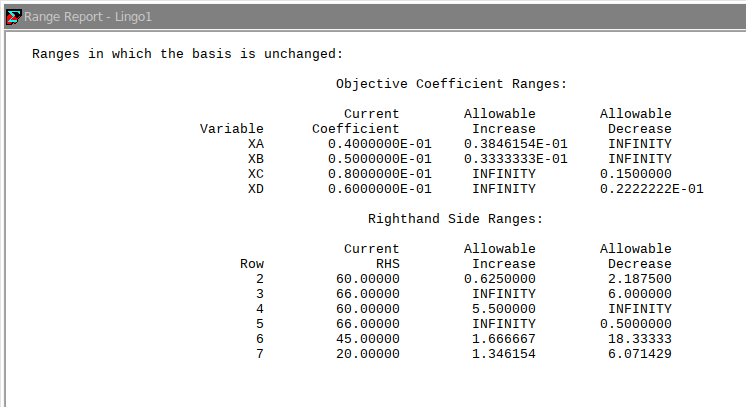
\includegraphics[width=0.95\linewidth]{Lindo tarefa 3 range a.png}
\caption{Análise de sensibilidade do modelo original. Na linha 2,
o aumento permitido para a dose mínima na borda é de $0{,}625$ Gy.}
\label{fig:tarefa3-range}
\end{figure}

O aumento da exigência na borda eleva o valor de $Z$, o que representa
uma piora em um problema de minimização. Isso sugere verificar o efeito
contrário, reduzindo essa exigência. Os testes realizados no LINDO
confirmaram a redução de $Z$. O próprio relatório permite explicar
esse comportamento. Na linha 2, a coluna \texttt{Allowable Decrease}
indica que o limite pode diminuir em até $2{,}1875$ Gy mantendo o
\textit{dual price} original. Assim, reduzir a dose mínima na borda de 60 para
59 Gy, mantendo os demais limites fixos, reduz a dose média no tecido
sadio em $0{,}30$ Gy,
\[
Z=5{,}50-0{,}30=5{,}20\text{ Gy}.
\]
Essa melhora no objetivo depende de aceitar uma exigência menor de
dose na borda do tumor, alterando o requisito original do problema.

\subsection*{Item (b)}

\textbf{Quanto se ganha afrouxando o limite da medula em 1 Gy?
E o do pulmão?}

Afrouxar o limite significa permitir mais dose no órgão. Como os \textit{dual price} das linhas 6 e 7 são positivos, esse aumento permite reduzir a
 dose média mínima no tecido sadio. Consideramos cada mudança
 separadamente, mantendo os demais limites do modelo original.

Na medula, o \textit{dual price} da linha 6 é $+0{,}10$ Gy/Gy. Aumentar o limite
 de 45 para 46 Gy proporciona um ganho de \textbf{0,10 Gy} no tecido sadio,
 cuja dose média passa a
\[
Z=5{,}50-0{,}10(1)=\boxed{5{,}40\text{ Gy}}.
\]
No pulmão, o \textit{dual price} da linha 7 é $+0{,}40$ Gy/Gy. Aumentar o limite
 de 20 para 21 Gy proporciona um ganho de \textbf{0,40 Gy} no tecido sadio,
 cuja dose média passa a
\[
Z=5{,}50-0{,}40(1)=\boxed{5{,}10\text{ Gy}}.
\]

\subsection*{Item (c)}

\textbf{Se o médico pudesse negociar 1 Gy em um dos dois limites,
qual escolheria? Até quantos Gy essa conta vale?}

Pelo objetivo do modelo, escolheria aumentar o limite do \textbf{pulmão}.
O ganho de $0{,}40$ Gy na dose média do tecido sadio é quatro vezes
maior que o ganho de $0{,}10$ Gy obtido ao aumentar o limite da medula.

Para saber até quando essa taxa vale, consultamos a linha 7 da análise
 de sensibilidade. O limite atual é 20 Gy e o aumento permitido é
 $1{,}346154$ Gy. Assim, a redução de $0{,}40$ Gy no tecido sadio por Gy
 adicional permitido no pulmão vale até o limite pulmonar chegar a
\[
20+1{,}346154\approx\boxed{21{,}3462\text{ Gy}}.
\]
Portanto, podemos usar o mesmo \textit{dual price} para um aumento total de até
\textbf{1,3462 Gy}, mantendo os demais limites fixos. Nesse ponto, o
feixe D chega à intensidade zero. Para aumentos maiores, é necessário
resolver novamente o modelo para determinar o novo ganho.

\clearpage
\section*{Tarefa 4 -- O feixe que ficou de fora}

\subsection*{Item (a)}

\textbf{O \texttt{REDUCED COST} do feixe C é $0{,}15$, maior que seu
próprio coeficiente ($0{,}08$). Que melhoria no tecido sadio faria
o feixe C entrar no plano?}

Como o problema é de minimização, o custo reduzido de $0{,}15$ indica
quanto o coeficiente de C na função objetivo precisa diminuir para
que esse feixe possa participar de uma solução ótima. O coeficiente
atual é $0{,}08$ Gy no tecido sadio por unidade de intensidade.
Portanto, ele precisaria chegar a
\[
0{,}08-0{,}15=\boxed{-0{,}07\text{ Gy por unidade de intensidade}}.
\]
Nesse valor, C pode entrar em uma solução ótima alternativa. Abaixo
dele, seu uso passa a ser vantajoso. Isso exigiria que o feixe reduzisse
a dose no tecido sadio, algo incompatível com a deposição de dose
representada pelo modelo. Mesmo reduzir seu coeficiente a zero
seria insuficiente.

\subsection*{Item (b)}

\textbf{Decomponha o $0{,}15$ usando a coluna de C e os \textit{dual price}.
Quanto vale a dose entregue à borda e quanto custam as doses na
medula e no pulmão? Qual é o verdadeiro obstáculo do feixe C?}

Cada unidade de intensidade de C entrega $0{,}9$ Gy à borda e deposita
$0{,}2$ Gy na medula, $0{,}8$ Gy no pulmão e $0{,}08$ Gy no tecido
sadio. Usando os \textit{dual price}, expressamos os benefícios e custos
em dose média equivalente no tecido sadio por unidade de intensidade de C.

\begin{center}
\begin{tabular}{llr}
\toprule
\textbf{Contribuição} & \textbf{Cálculo} & \textbf{Efeito (Gy/unidade)} \\
\midrule
Benefício na borda & $0{,}9\times0{,}30$ & $-0{,}27$ \\
Custo na medula & $0{,}2\times0{,}10$ & $+0{,}02$ \\
Custo no pulmão & $0{,}8\times0{,}40$ & $+0{,}32$ \\
Dose direta no tecido sadio & $0{,}08$ & $+0{,}08$ \\
\bottomrule
\end{tabular}
\end{center}

O benefício na borda é subtraído porque essa dose ajuda a cumprir a
exigência mínima do tumor. As doses na medula e no pulmão consomem
limites já atingidos e entram como custos. As demais restrições têm
\textit{dual price} zero. Assim,
\[
\text{Custo reduzido de C}
=0{,}08-0{,}27+0{,}02+0{,}32
=\boxed{0{,}15\text{ Gy por unidade de intensidade}}.
\]

O principal obstáculo é a \textbf{dose depositada no pulmão}.
Seu custo equivalente de $0{,}32$ Gy já supera o benefício de
$0{,}27$ Gy na borda. Somados os custos da medula e do tecido sadio,
o feixe C piora o valor da função objetivo.

\clearpage
\section*{Tarefa 5 -- Um pulmão frágil}

\subsection*{Item (a)}

\textbf{Com limite de 18 Gy e de 15 Gy, qual a dose média no tecido
sadio? Use só o relatório.}

Na linha 7 do relatório, o limite pulmonar original é 20 Gy e o
\textit{dual price} é $+0{,}40$. Portanto, reduzir esse limite aumenta
a dose média mínima no tecido sadio em $0{,}40$ Gy por Gy retirado
do limite pulmonar, mantendo as demais exigências fixas.

A coluna \texttt{Allowable Decrease} da
Figura~\ref{fig:tarefa3-range} permite uma redução de até
$6{,}071429$ Gy. As reduções para 18 Gy e 15 Gy são de 2 Gy e
5 Gy, respectivamente, e estão dentro desse intervalo. Assim,
podemos usar o relatório original, sem resolver novamente o modelo.

Para o limite de \textbf{18 Gy}, a dose média no tecido sadio é
\[
Z=5{,}50+0{,}40(20-18)=\boxed{6{,}30\text{ Gy}}.
\]
Para o limite de \textbf{15 Gy}, essa dose passa a ser
\[
Z=5{,}50+0{,}40(20-15)=\boxed{7{,}50\text{ Gy}}.
\]

\subsection*{Item (b)}

\textbf{Com 12 Gy, o que o LINDO responde? O que isso significa para
o tratamento?}

Ao reduzir o limite pulmonar para 12 Gy, o programa apresenta o estado
\texttt{Infeasible} e a mensagem \texttt{No feasible solution found}.
Isso significa que nenhuma combinação dos quatro feixes atende
simultaneamente às doses exigidas no tumor, ao limite de 45 Gy na
medula e ao limite de 12 Gy no pulmão. Portanto, o plano de tratamento
é inviável nas condições desse modelo.

O valor $8{,}25$ exibido em \texttt{Objective} pertence a uma tentativa
que viola restrições e não representa a dose de um plano viável.

\begin{figure}[H]
\centering
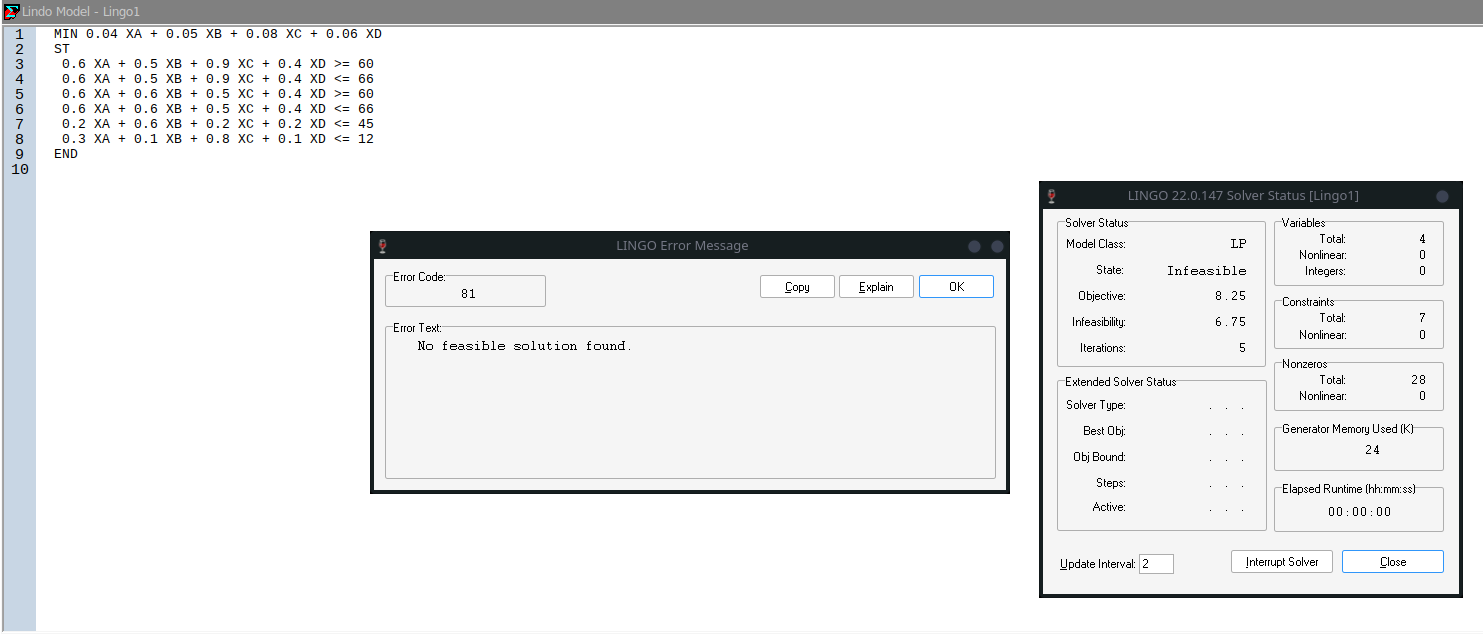
\includegraphics[width=0.95\linewidth]{Lindo tarefa 5 no feasible.png}
\caption{Execução do modelo PPL no LINDO com limite de 12 Gy no pulmão.
O programa indica que não há solução viável.}
\label{fig:lindo-tarefa-5-nofeasible}
\end{figure}

\subsection*{Item (c)}

\textbf{Qual a menor dose no pulmão com que ainda se trata o tumor
(60 Gy, medula até 45 Gy)? Monte e resolva no LINDO o PPL que responde
a essa pergunta.}

Para descobrir a menor dose média possível no pulmão, usamos os
coeficientes da linha do pulmão na tabela do enunciado para montar
a nova função objetivo,
\[
\min D_{\text{pulmão}}=0{,}3x_A+0{,}1x_B+0{,}8x_C+0{,}1x_D.
\]
As variáveis continuam representando as intensidades não negativas
dos quatro feixes. Mantemos as doses na borda e no centro entre 60 e
66 Gy, conforme o problema original, e a medula com no máximo 45 Gy.
Essas restrições garantem que o plano atenda às exigências do tumor
e da medula enquanto a dose no pulmão é minimizada.

Retiramos a restrição que fixava um máximo para o pulmão, pois agora
queremos que o programa encontre sua menor dose possível. No LINDO,
o novo modelo é
\begin{center}
\begin{minipage}{0.5\linewidth}
\begin{verbatim}
MIN 0.3 XA + 0.1 XB + 0.8 XC + 0.1 XD
ST
 0.6 XA + 0.5 XB + 0.9 XC + 0.4 XD >= 60
 0.6 XA + 0.5 XB + 0.9 XC + 0.4 XD <= 66
 0.6 XA + 0.6 XB + 0.5 XC + 0.4 XD >= 60
 0.6 XA + 0.6 XB + 0.5 XC + 0.4 XD <= 66
 0.2 XA + 0.6 XB + 0.2 XC + 0.2 XD <= 45
END
\end{verbatim}
\end{minipage}
\end{center}

A solução ótima indica que a menor dose média no pulmão é de aproximadamente 13,93 Gy, 
respeitando as exigências do tumor e o limite da medula.

\begin{figure}[H]
\centering
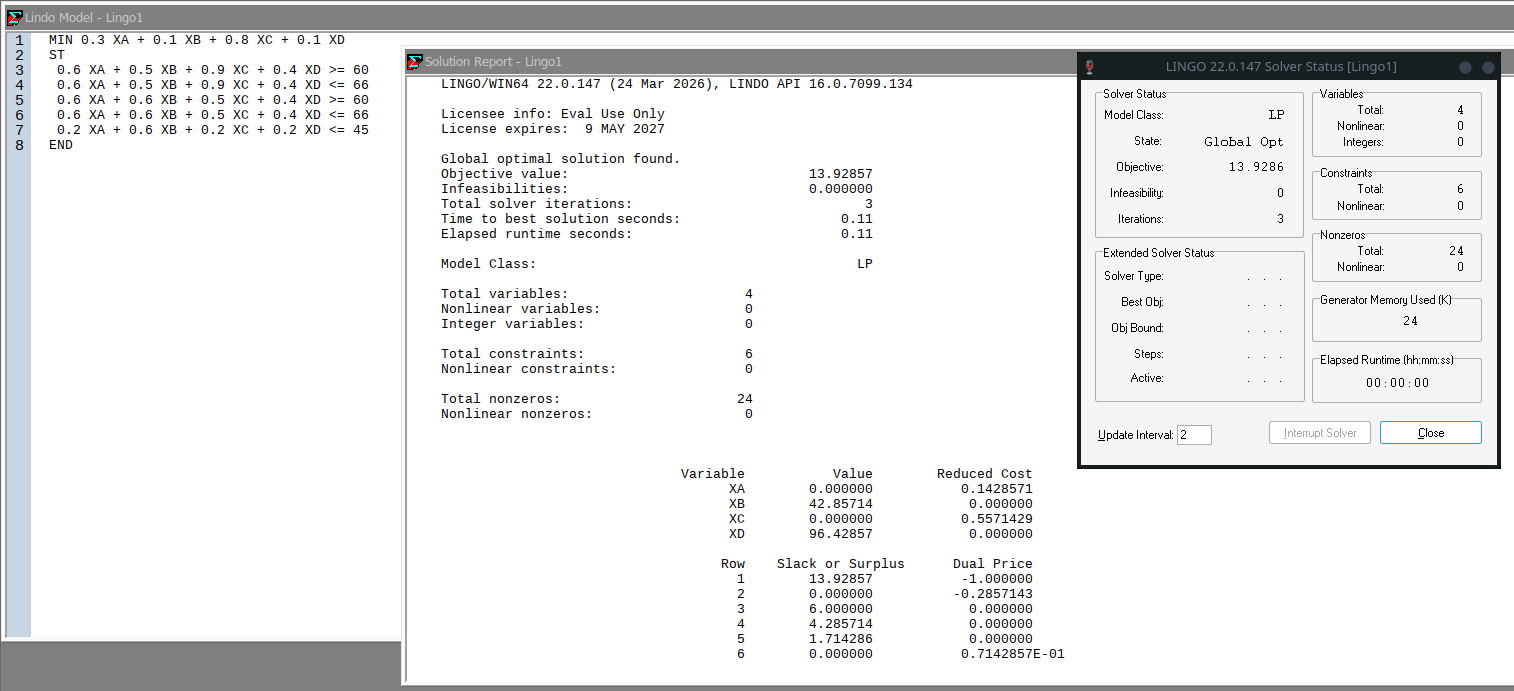
\includegraphics[width=0.95\linewidth]{lindo tarefa 5 novo ppl.png}
\caption{Solução do PPL que minimiza a dose média no pulmão.}
\label{fig:tarefa5-c}
\end{figure}

\subsection*{Item (d)}

\textbf{Faça o gráfico da dose média no tecido sadio em função do limite
do pulmão, desse mínimo até 26 Gy.}

Para construir o gráfico, usamos o modelo original, que minimiza a
 dose média no tecido sadio, variando apenas o limite pulmonar.
 Com esse limite em 26 Gy, o LINDO fornece $Z=4{,}444444$ Gy e
 \textit{dual price} de $0{,}1111111$ na linha 7.

\begin{figure}[H]
    \centering
    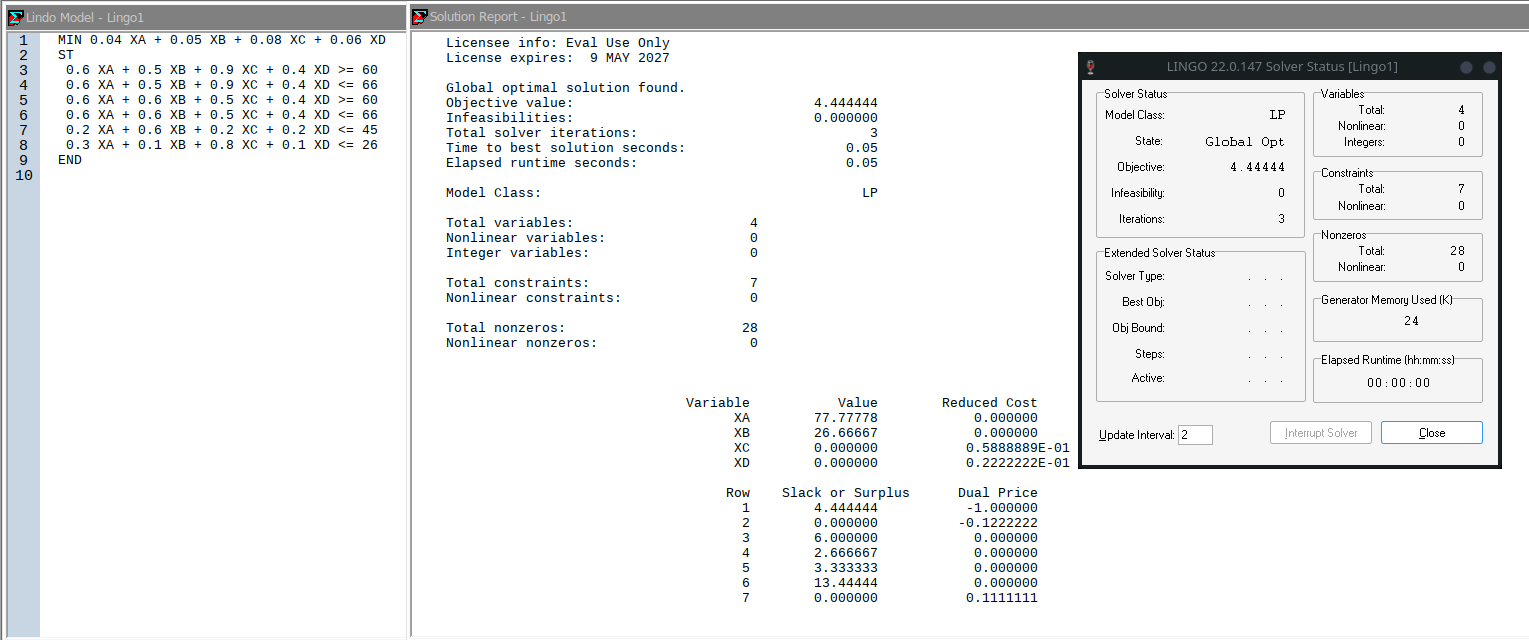
\includegraphics[width=0.95\linewidth]{lindo tarefa 5 D solver.png}
    \caption{Solução ótima com limite pulmonar de 26 Gy.}
    \label{fig:tarefa5-d-solver}
\end{figure}

No relatório original, o limite de 20 Gy pode diminuir em
$6{,}071429$ Gy ou aumentar em $1{,}346154$ Gy. Nesse intervalo,
a dose ótima no tecido sadio é calculada por
\[
Z(L)=5{,}50-0{,}40(L-20),
\qquad 13{,}928571\leq L\leq21{,}346154,
\]
onde $L$ representa o limite pulmonar, em Gy.

Já no relatório com limite de 26 Gy, a linha 7 apresenta
\texttt{Allowable Decrease} de $4{,}653846$ Gy. Portanto, o novo
\textit{dual price} vale desde $26-4{,}653846=21{,}346154$ Gy,
ligando-se ao primeiro intervalo. Para esse segundo trecho,
\[
Z(L)\approx4{,}444444+0{,}1111111(26-L),
\qquad21{,}346154\leq L\leq26.
\]
Os valores estão arredondados conforme os relatórios.

\begin{figure}[H]
    \centering
    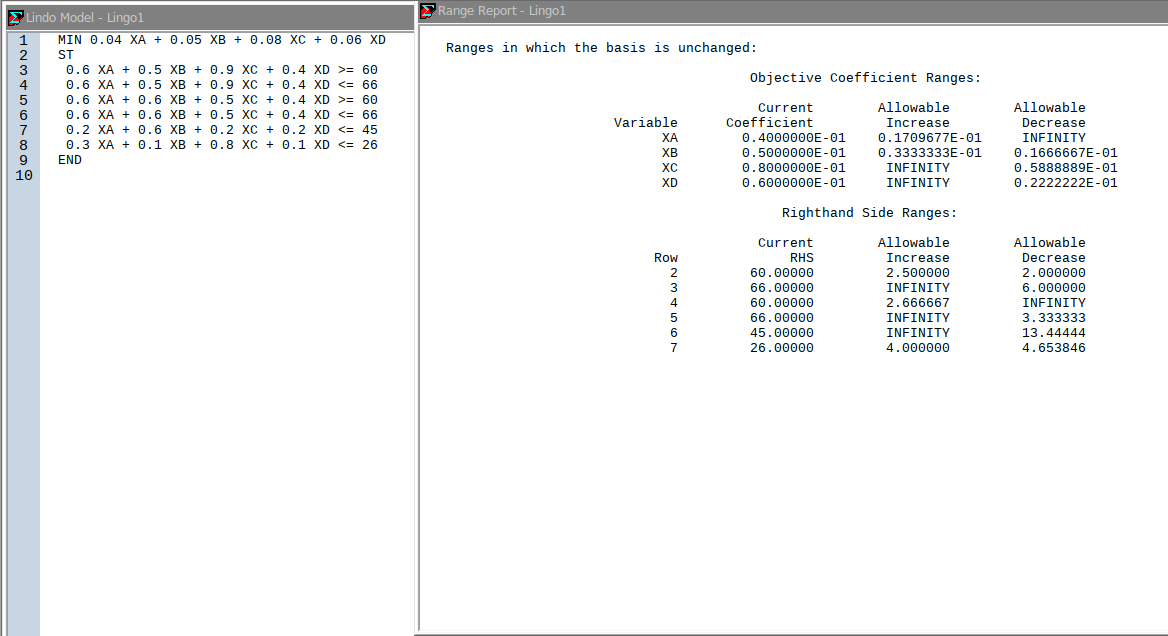
\includegraphics[width=0.95\linewidth]{lindo tarefa 5 D range report.png}
    \caption{Análise de sensibilidade com limite pulmonar de 26 Gy.}
    \label{fig:tarefa5-d-range}
\end{figure}

Como cada intervalo tem uma taxa constante, o gráfico é formado por
 dois segmentos de reta. Os extremos usados são
\begin{center}
\begin{tabular}{rr}
\toprule
\textbf{Limite pulmonar (Gy)} & \textbf{Dose ótima no tecido sadio (Gy)} \\
\midrule
$13{,}928571$ & $7{,}928571$ \\
$21{,}346154$ & $4{,}961538$ \\
$26{,}000000$ & $4{,}444444$ \\
\bottomrule
\end{tabular}
\end{center}
Os dois primeiros valores de dose foram calculados pela expressão
 do primeiro trecho, e o último veio da execução com 26 Gy.
 O script em Python usa o Seaborn apenas para representar esses pontos
 e ligá-los com segmentos de reta.

\begin{figure}[H]
    \centering
    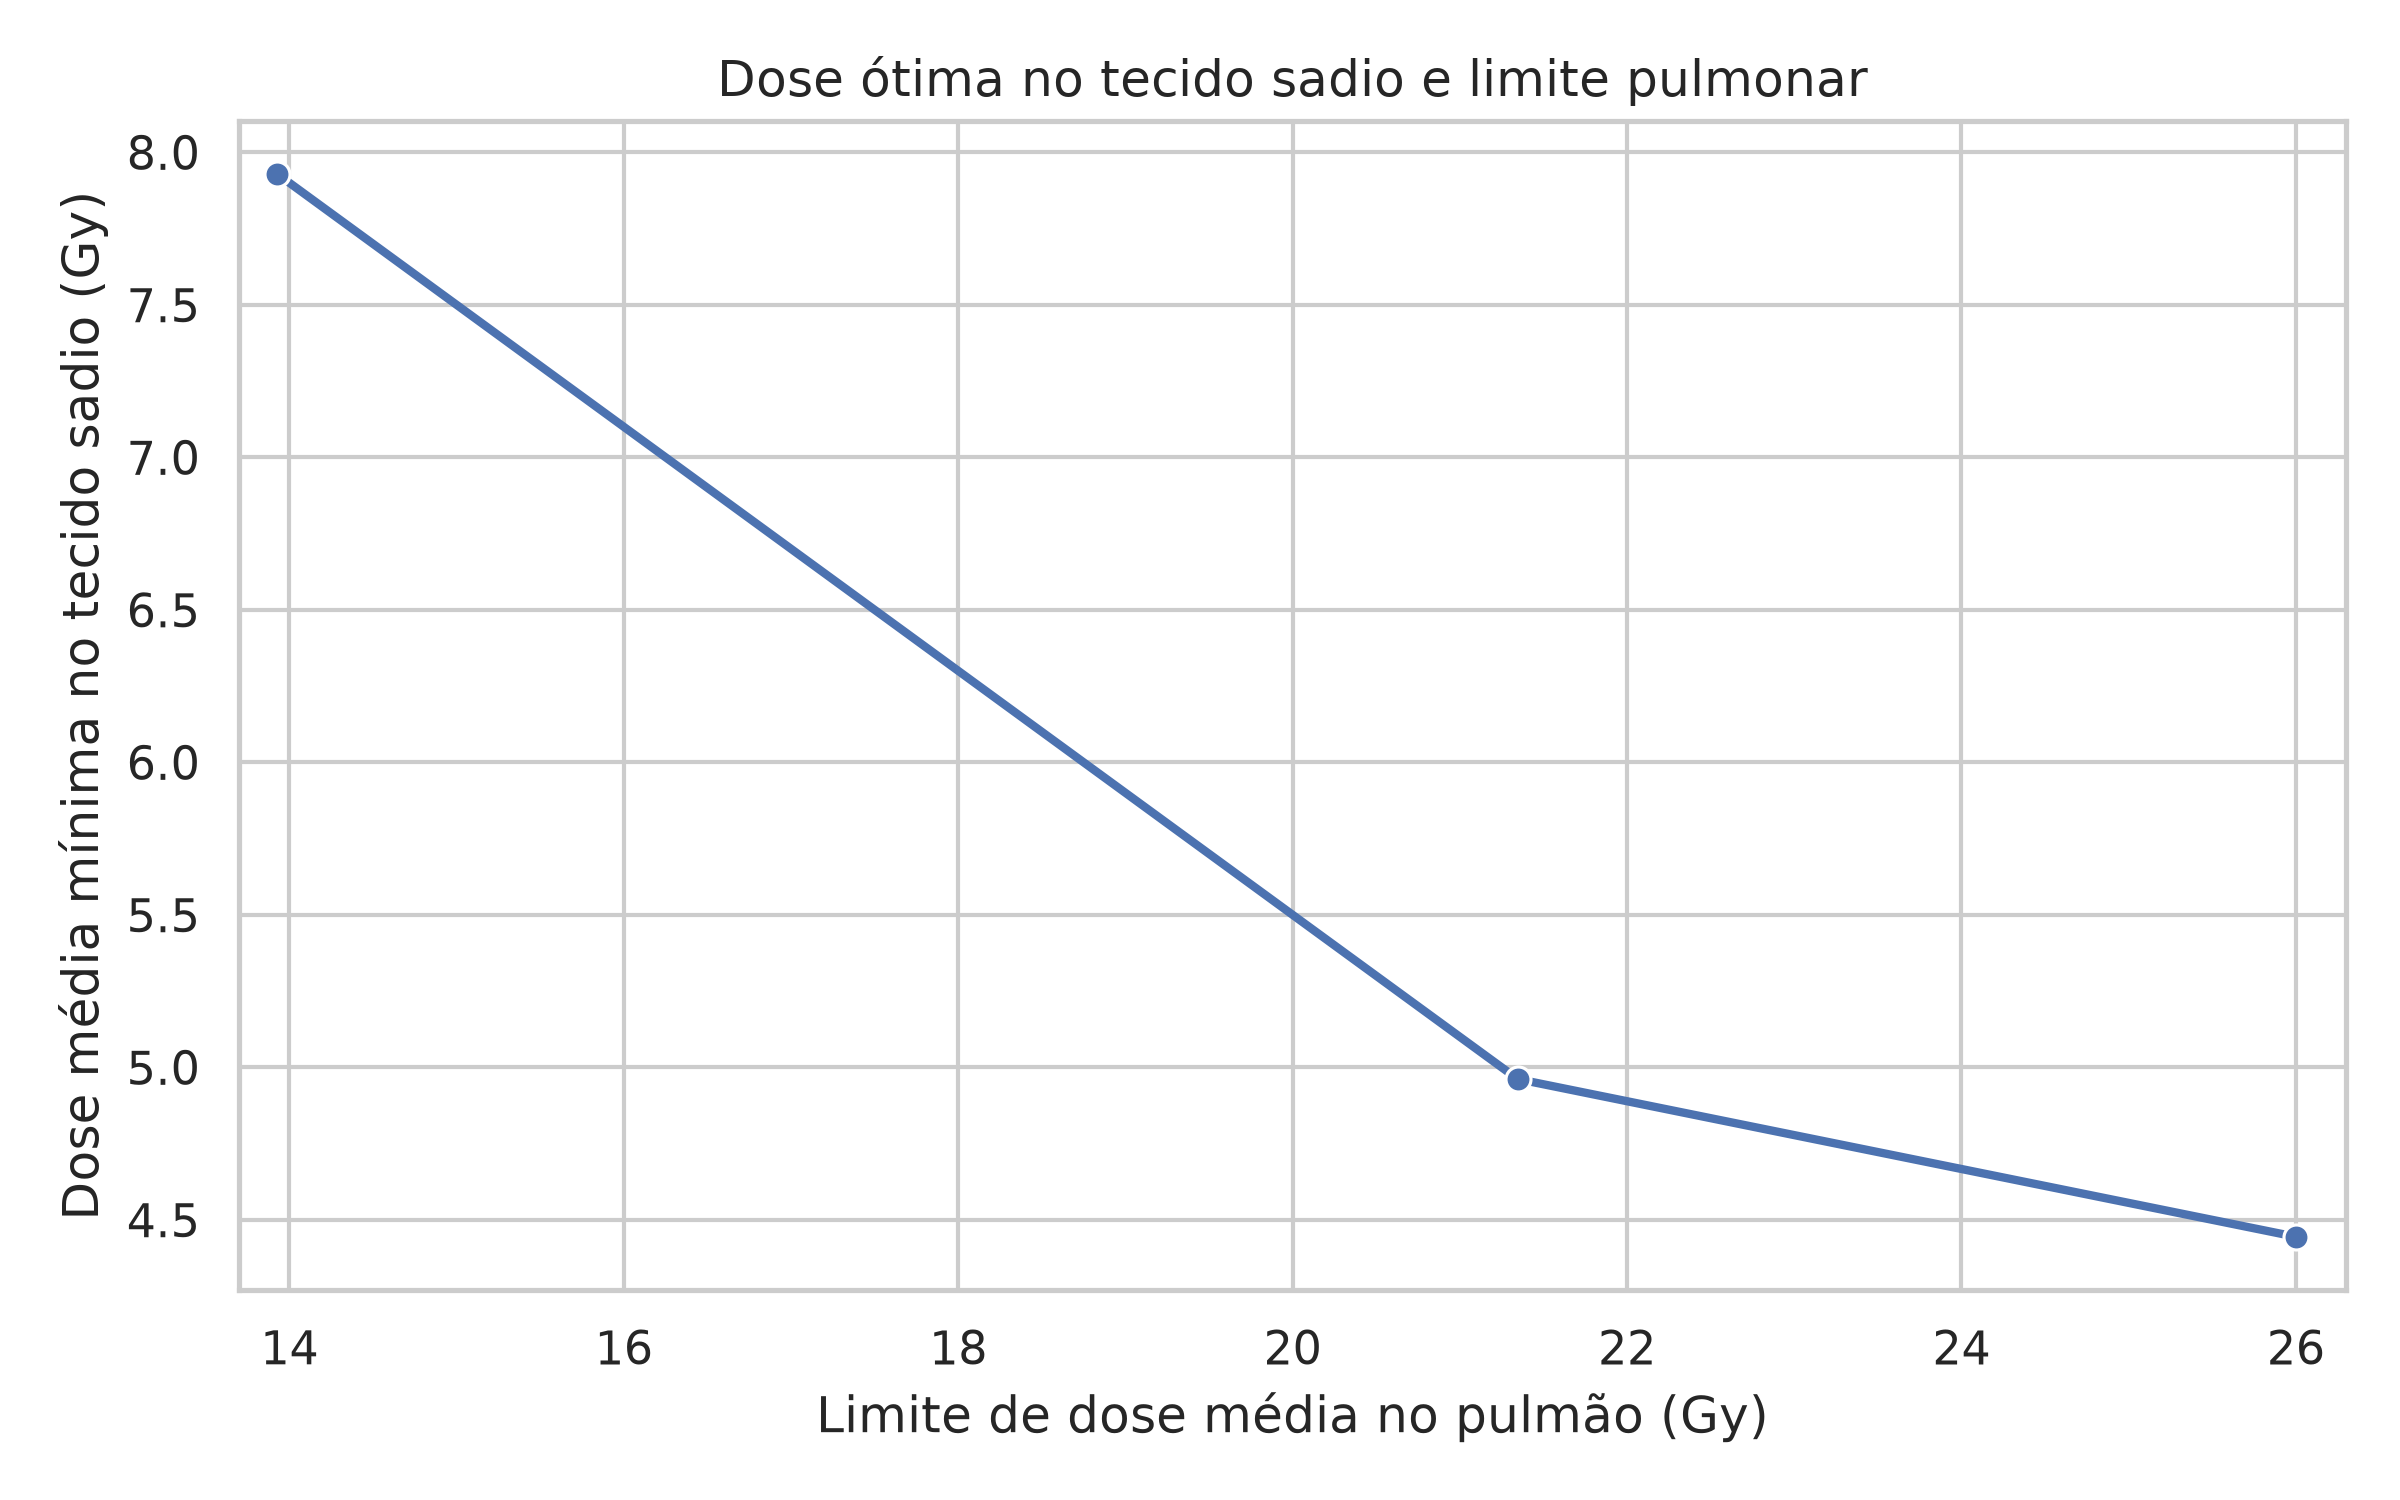
\includegraphics[width=0.8\linewidth]{grafico_tarefa5.png}
    \caption{Dose média mínima no tecido sadio em função do limite pulmonar.}
    \label{fig:tarefa5-d}
\end{figure}

A dose ótima no tecido sadio diminui conforme o limite pulmonar
 aumenta. A mudança de inclinação em aproximadamente $21{,}3462$ Gy
 corresponde à redução do ganho por Gy adicional permitido no pulmão,
 de $0{,}40$ para aproximadamente $0{,}1111111$ Gy.

\end{document}
